\chapter{Introducci\'on}
\label{chap:introduccion}

\par \textbf{SidelabCode Stack} es una forja de desarrollo de Software para su uso como herramienta \textbf{ALM}. Es una herramienta FLOSS (Free Libre Open Source Software) con Licencia \textbf{TBC}.

\begin{figure}[h]
    \begin{center}	
        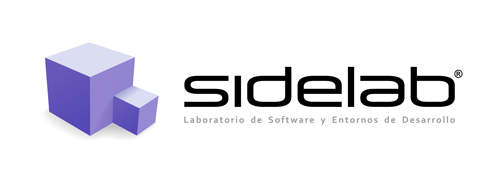
\includegraphics[width=1\textwidth]{sidelab}
        \label{fig:sidelab}
    \end{center}
\end{figure}

\par El desarrollo de este proyecto se basa en el dise\~no e implementaci\'on del proceso de desarrollo acorde con las metodolog\'ias \'agiles a trav\'es de la forja \emph{SidelabCode Stack}. Unificando herramientas a trav\'es de las distintas APIs basadas en la interoperabilidad, facilitando la instalaci\'on, la replicaci\'on y la recuperaci\'on de los datos mediante el uso de Software Libre para construir Software de calidad.

\par El uso de metodolog\'ias \'agiles se encuentra intr\'insecamente relacionado a lo largo del proceso de desarrollo e implementaci\'on de la forja. Por otra parte podemos afirmar que no es una herramienta intrusiva para la aplicaci\'on de las distintas metodolog\'ias ligadas a un proceso de desarrollo.

\par Presentando las distintas metodolog\'ias de desarrollo de software definidas analizando sus caracter\'isticas tanto las buenas como las malas y como \'estas se aplican al dise\~no de la herramienta encaminado un proceso de desarrollo fluido y \'agil para un desarrollador o un grupo de desarrolladores.

\par Un punto a tener en cuenta es la ergonom\'ia con la que cuenta la herramienta para el d\'ia a d\'ia y las soluciones que aporta con respecto a otras herramientas que cohabitan en el mismo campo.

\par Todo con un mismo fin; producir software de calidad evaluable, es decir, no es necesario crear un producto perfecto sino se sabe mejorarlo y adaptarlo a nuevas necesidades. Para eso utilizamos las herramientas ALM en los proyectos ya que nos ayudan a tener una visi\'on diaria y a posteriori con perspectiva para poder medir y evaluar las mejoras entre dos puntos de tiempo. Por lo tanto \emph{la evoluci\'on del proyecto y la adaptabilidad a los cambios}.

\section{Etimolog\'ia}
\label{sec:etimologia}

\par Sidelab es, un laboratorio de software. Partiendo de esta base, encontramos una definici\'on exacta para SidelabCode \footnote{\url{http://code.sidelab.es/projects/sidelab/wiki/Sidelab}}:

\begin{quotation}
        \emph{Sidelab es el "laboratorio de software y entornos de desarrollo integrados" (Software and Integrated Development Environments Laboratory). Es un grupo de entusiastas de la programaci\'on con inter\'es en pr\'acticamente todos los aspectos del desarollo, desde los lenguajes de programaci\'on y los algoritmos avanzados, hasta la ingenier\'ia del software y la seguridad inform\'atica. Nuestros principales intereses se centran en el desarrollo software y la mejora y personalizaci\'on de los entornos de desarrollo integrados (IDEs) y herramientas relacionadas.}
\end{quotation}

\par En el otro extremo del nombre se encuentra \emph{Code} se refiere al c\'odigo en s\'i hacia donde se orienta esta herramienta. Por ultimo pero no menos importante tenemos \emph{Stack}, es una pila de servicios para la gesti\'on y el desarrollo de proyectos software.

\par Como resultado tenemos \textbf{SidelabCode Stack} una Forja de desarrollo de aplicaciones orientada a un proceso de desarrollo.

% subsection etimologia (end)

\section{Trabajo en TSCompany}
\label{sec:trabajo-tscompany}

\par Explicaci\'on del trabajo efectuado en TSCompany durante el desarrollo de la implementaci\'on de la Forja.

\par El pr\'acticum del M\'aster me dio la oportunidad de entrar a trabajar en la empresa TSCompany para cubrir la plaza de becario. Desde el principio he estado interesado en la producción de software de calidad, en las herramientas e control de versiones, el desarrollo orientado a tests, la documentación y de como unificar las herramientas para obtener un rendimiento óptimo a la hora de desarrollar un proyecto, es decir, un desarrollador que desarrollar al 100\%.

\par Esta colaboraci\'on se bas\'o en la aportaci\'on al proyecto de \emph{Software Libre} SidelabCode Stack.

\par Profesionalmente siempre he tenido ejemplos cercanos acerca del desarrollo de software de calidad y me ha han inculcado el desarrollo orientado a tests \emph{TDD}. Siempre he perseguido la simplicidad y de esta forma la replicaci\'on de un entorno, pruebas, instalaciones y la estandarizaci\'on de la programaci\'on para una comprensi\'on sencilla.

\par El objetivo inicial era pulir el funcionamiento de la herramienta SidelabCode Stack unificando el proceso de desarrollo en la instalaci\'on ya que hab\'ian m\'odulos que todav\'ia no estaban controlados, es decir, centralizados y quedaban dispersos para el usuario final. Por ejemplo, el usuario ten\'ia que ejecutar una serie pasos para poder incluir un proyecto en un repositorio distribuido Git.

\par Hab\'ia que dar forma al modelo de desarrollo y promocionarlo dentro de la estructura de la forja para que resultase f\'acil para el usuario empezar a desarrollar su proyecto dentro del entorno SidelabCode.

\par Despu\'es de la formalizaci\'on de las distintas versiones del proyecto, se invirti\'o un tiempo para la implantaci\'on de la forja en la empresa TSCompany para su uso diario. Partiendo de la migraci\'on de la informaci\'on de todos los proyectos y usuarios de la empresa para as\'i poder gestionarlos a trav\'es de un interfaz com\'un, SidelabCode Stack. Debido al uso de herramientas de Software Libre la migraci\'on fue fluida y nada agresiva para los usuarios. El entorno de trabajo segu\'ia siendo el mismo pero en este caso aportando un extra de calidad y m\'etricas para la evaluaci\'on de los proyectos desarrollados.

% subsection trabajo-tscompany (end)